\documentclass[tikz,border=8pt]{standalone}
\usepackage{amsmath}
\usetikzlibrary{decorations.pathreplacing}

\begin{document}
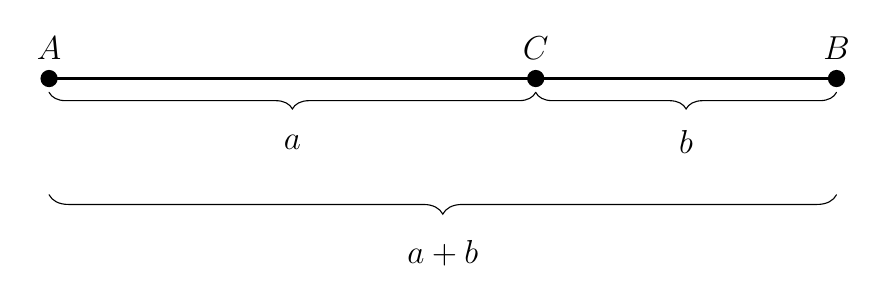
\begin{tikzpicture}[
  line cap=round,
  every node/.style={font=\large},
  point/.style={circle,fill=black,inner sep=2.2pt}
]
  \coordinate (A) at (0,0);
  \coordinate (C) at (6.18,0);
  \coordinate (B) at (10,0);

  \draw[very thick] (A) -- (B);
  \node[point,label=above:$A$] at (A) {};
  \node[point,label=above:$C$] at (C) {};
  \node[point,label=above:$B$] at (B) {};

  \draw[decorate,decoration={brace,mirror,amplitude=6pt}]
    ([yshift=-5pt]A) -- ([yshift=-5pt]C)
    node[midway,yshift=-18pt] {$a$};

  \draw[decorate,decoration={brace,mirror,amplitude=6pt}]
    ([yshift=-5pt]C) -- ([yshift=-5pt]B)
    node[midway,yshift=-18pt] {$b$};

  \draw[decorate,decoration={brace,mirror,amplitude=7pt}]
    ([yshift=-42pt]A) -- ([yshift=-42pt]B)
    node[midway,yshift=-21pt] {$a+b$};
\end{tikzpicture}
\end{document}
